\subsection{League of Legends - previsão baseada nos 10 primeiros minutos de jogo}
    \subsubsection{Principais nodos}
        \begin{figure}[H]
            \centering
            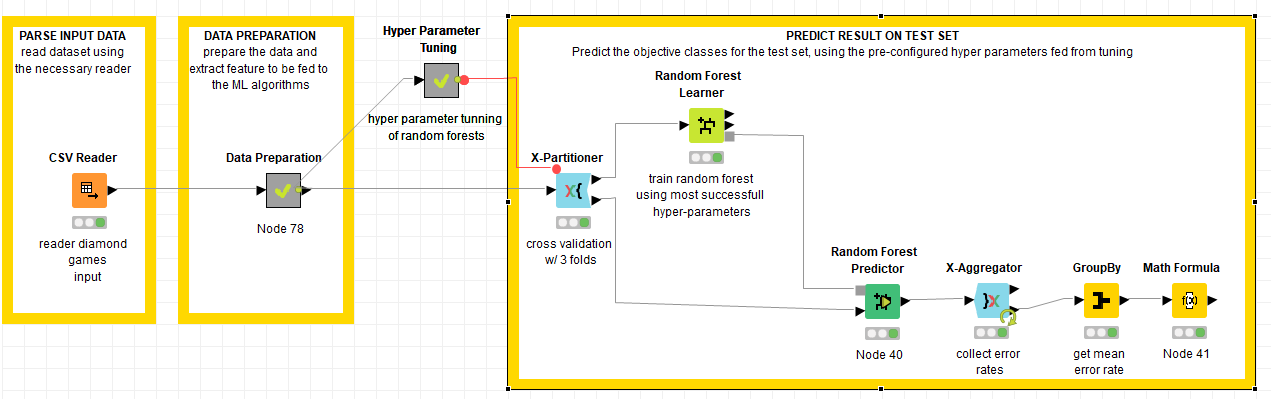
\includegraphics[scale=0.30
            ]{Figures/wf_lol.png}
            \caption{Visão geral do workflow gerado para trabalhar o dataset.}
            \label{fig:"um"}
        \end{figure} 
        
    \begin{enumerate}
        \item \textbf{Parse Input Data} \\
            Como ponto inicial do nosso processo tivemos que ler os dados a serem utilizados. Os dados originais encontravam-se num ficheiro .csv, assim sendo utilizamos o nodo CSV Reader.
        
        \item \textbf{Data Preparation} \\
            Após carregados os dados, passamos ao tratamento/preparação dos mesmos. Para tal desenvolvemos o workflow presente na figura abaixo.
            \begin{figure}[H]
                \centering
                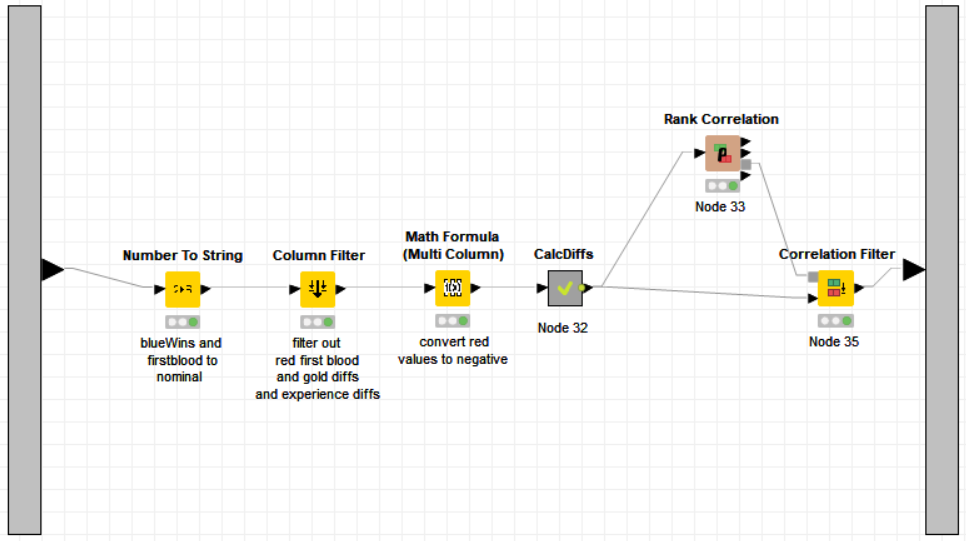
\includegraphics[scale=0.30
                ]{Figures/wf_lol_data.png}
                \caption{Visão geral do workflow gerado para trabalhar o dataset.}
                \label{fig:"um"}
            \end{figure} 
            Os dados presentes em cada registo, como já referido antes, eram bastante redundantes, uma vez que o \textit{dataset} possuía todos os dados para ambas as equipas. Desta forma optámos por transformar estes dados num diferencial. Como exemplo, no \textit{dataset}, antes do tratamento, tínhamos dados como o número de mortes que a equipa azul causou e o número de mortes que a equipa vermelha causou. Depois deste processo deixamos de ter estas duas colunas e passamos a ter uma variável que indica a diferença entre o número de mortes causadas por cada equipa. Por fim aplicamos um \textit{correlation filter}, com um \textit{treshold} de quase 1, de forma a eliminar automaticamente as colunas que podiam praticamente ser obtidas a partir das restantes, como por exemplo a diferença entre o número de jogadores mortos pelas equipas e a diferença de vezes que cada equipa morreu.
        
        \item \textbf{Hyper Parameter Tuning} \\
            Para fazermos o tuning utilizamos o metanodo que previamente desenvolvemos para treinar o modelo para a competição de \textit{Kaggle}. Desta forma o funcionamento do mesmo não será explicitado neste ponto, uma vez que seria repetitivo.
        \item \textbf{Previsões} \\
            A partir do momento que temos os parâmetros óptimos para o nosso modelo podemos finalmente treinar e testar o mesmo. Para tal utilizamos o nodo "X Partitioner", utilizando 3 folds. Uma vez terminado este processo calculamos a precisão do modelo, considerando que o método de agrupamento dos resultados nos retorna a média do erro entre as 3 folds.
    \end{enumerate}
        
    \subsubsection{Descrição do modelo gerado}
        \begin{enumerate}
            \item \textbf{Tuning}\\
                Pelo motivo referido acima, não iremos entrar em detalhe neste ponto. Existe uma descrição detalhada do mesmo nos pontos 4.1.1 e 4.1.2
            \item \textbf{Características do treino}\\
                Após terminado o loop de optimização temos então os valores óptimos para a nossa \textit{Decision Tree}. No caso em concreto os parâmetros "ideais" foram os seguintes:
                \begin{itemize}
                    \item Número de modelos: 500
                    \item Profundidade da árvore: 10
                    \item Split Criterions: Information Gain
                \end{itemize}
                \begin{figure}[H]
                    \centering
                    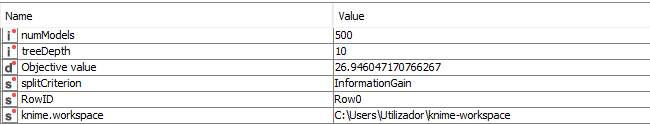
\includegraphics[scale=0.30
                    ]{Figures/wf_lol_hyperdata.png}
                    \caption{Settings utilizados para treino do modelo.}
                    \label{fig:"um"}
                \end{figure} 
        \end{enumerate}